\section{Assembler Addressing \& Programming}

\subsection{Assembler Instructions}

\textit{
    There are 3 main type of instructions:
}

\begin{itemize}
    \item{Data \textbf{Transport}}
    \item{\textbf{Operations} (Arithmetic, Logic, Bit-manipulation, Shift and Rotation)}
    \item{Program \textbf{Branches} with jump and branch operations}
\end{itemize}

\subsection{Transport Operations}

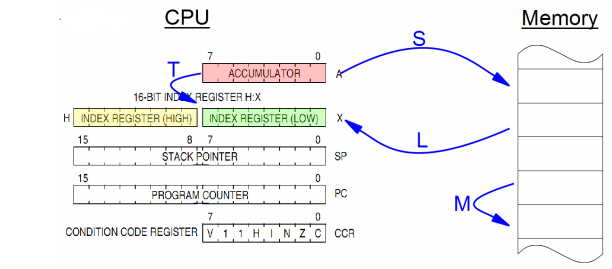
\includegraphics[width=0.5\textwidth]{transport-operations.png}

\begin{tabular}{llp{0.3\textwidth}}
      & \textbf{Operation} & \textbf{Example} \\
    L & Load     & \textit{LDA, LDX, LDHX; PULA, PULX (Stackoperations)} \\
    S & Store    & \textit{STA, STX, STHX; PSHA, PSHZ (Stackoperations)} \\
    T & Transfer & \textit{TAP, (CCR = Accu.), TPA, TAX, TSX} \\
    M & Move     & \textit{MOV} \\
\end{tabular}

\subsection{Arithmetic Operations}

\begin{tabular}{lp{0.38\textwidth}}
    \textbf{ADD} & \textit{Adds given operand to the ACC.} \\
    \textbf{SUB} & \textit{Works equivalent to the addition.} \\
    \textbf{ADC} \& \textbf{SBC}
                & \textit{
                    Include Carry bit and support additions and subtractions
                    with numbers with more then 8 bits.
                } \\
    \textbf{MUL}
                & \textit{
                    Multiplies the content of the accumulator A with the content
                    of the index register X and stores the 16-bit result in X:A
                    (MSB in X, LSB in A)
                    \newline
                    \textbf{only unsigned}.
                } \\
    \textbf{DIV}
                & \textit{
                    divides the 16-bit dividend in H:A (MSB in H, LSB in A) with
                    the divisor in the index register X. The 8-bit result is written
                    to A. If an overflow or division by 0 occurs, the Carry-bit is set.
                    \newline
                    \textbf{only unsigned}.
                } \\
\end{tabular}

\textit{
    Results of arithmetic instructions are saved on the HCS08
    eather in the X-Register or AKKU
}

\subsection{Flags}

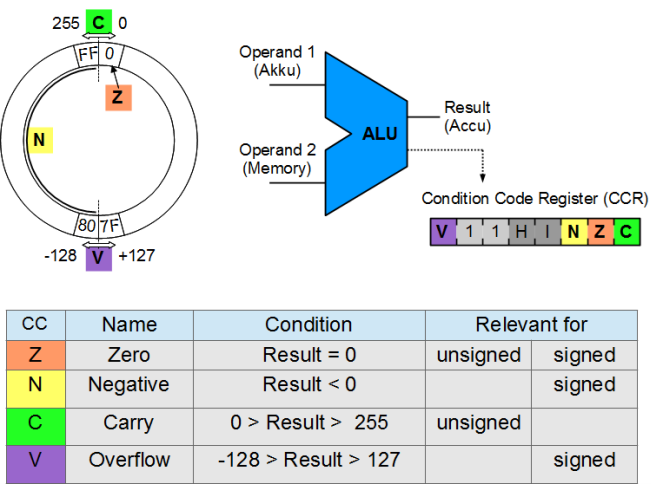
\includegraphics[width=0.5\textwidth]{instruction-flags}

\textit{\textbf{Half-Carry} is used for binary-coded decimal calculations}
\\
\begin{tabular}{ll}
    \textbf{ADD instruction} & \textbf{SUB instruction} \\
    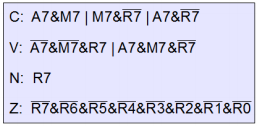
\includegraphics[width=0.24\textwidth]{flags-from-add.png} &
    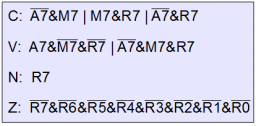
\includegraphics[width=0.24\textwidth]{flags-from-sub.png} \\
    A (Operand 1) \\
    M (Operand 2) \\
    R (Result 1) \\
\end{tabular}
